% anexo_a.tex

\chapter{Anexos}
\label{}



\section{Ejemplo Suma ponderada}\label{ej:sumapond}

Se tienen 3 escenarios posibles con $w = 1,2,3$ y parámetros $c_{w}= c_1,c_2,c_3$ y variables de diseño $x_{w}=x_{1}$, $x_{2}$,$x_{3}$. Luego, se tiene una suma ponderada de escenarios  $E_{\Theta}$[$x_{w}$ $c_{w}$] y la probabilidad de ocurrencia de cada escenario w es igual a $\Theta ={0.5 , 0.3 ,0.2 }$.
\vspace{2.5mm}

Con esto se tiene la siguiente expresión:

$$E_{\Theta} [ x_{w} c_{w}] = x_{1}c_{1}0.5 + x_{2}c_{2}0.3 + x_{3}c_{3}0.2 $$

\section{Parámetros Modelo Original}\label{anexo:parametros}


\section{Pruebas iniciales del rendimiento y atención racional en el subastador}\label{anexo:rendimiento}


Para realizar la evaluación del modelo, se realizará un gráfico con los resultados similar a la figura \ref{fig:fig6}. En esta se grafica la cantidad de permisos vendidos por el productor que produce energía con carbón y su influencia en el precio de mercado de los permisos. Esto representa el impacto que puede tener el modelo en eliminar el carbón como productor.

\begin{figure}[H]
    \centering
    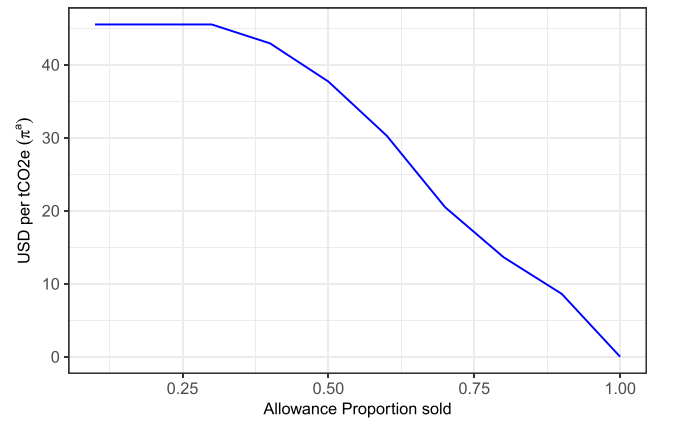
\includegraphics[width=15cm]{docs/DocumentoMemoria/images/figura 6 amigo.png}
    \caption{Venta de permisos por generador de carbón (Fuente: \protect\citeB{amigo_two_2021})}
    \label{fig:fig6}
\end{figure}


\subsubsection{Modelo sin restricciones}

Primero se evaluará el modelo al considerar únicamente la función objetivo del subastador con el costo original $\mathcal{F}$ y el costo de rendimiento. También se considera como variable de decisión únicamente los permisos $\theta$.  

\begin{equation}
\begin{array}{rrclcl}
    \displaystyle \min_{\theta} & -\theta \pi^aP + \tilde{\mathcal{F}}(P)+F(\theta)  \label{fo:perfornorest}\\
\end{array}
\end{equation}
\begin{equation}
\begin{array}{cl}
    \theta \geq 0 & (\varrho)\label{res:sub2}
\end{array}
\end{equation}

Con lo anterior se logra el siguiente Lagrangiano:

$$\mathcal{L}(\theta)=-P\theta\pi^a+\mathcal{F}(\theta)+c(P-d)^2 - \varrho\theta $$

Realizando la derivada de primer orden para $\theta$ se obtiene:

\begin{equation}
\begin{array}{rrclcl}
    \frac{\partial\mathcal{L}(\theta)}{\partial (\theta)}=-P\pi^a+\frac{\partial\mathcal{F}(\theta)}{\partial(\theta)}-\varrho=0 \label{lag1}\\
\end{array}
\end{equation}
\begin{equation}
\begin{array}{rrclcl}
    \rightarrow -P\pi^a+\frac{\partial\mathcal{F}(\theta)}{\partial(\theta)}=\varrho \label{lag1}\\
\end{array}
\end{equation}
Con esto se obtiene la siguiente complementariedad para el problema del subastador:

\begin{equation}
\begin{array}{rrclcl}
    0\leq -P\pi^a+\frac{\partial\mathcal{F}(\theta)}{\partial(\theta)}\perp \theta \geq 0 \label{compllag1}\\
\end{array}
\end{equation}

Al igual que en el modelo original de \citeB{amigo_two_2021}, se consideran los siguientes valores para constantes y parámetros:
\begin{enumerate}
    \item $\frac{\partial\mathcal{F}(\theta)}{\partial(\theta)}=0$
    \item $CAP\sim \mathcal{N}(100MtCO_{2}e,0)$
\end{enumerate}

Con esto, al correr el modelo en el \textit{solver}, cambiando únicamente el valor del rendimiento ($P$), se encontraron los siguientes resultados:

\begin{table}[H]
\centering
\begin{tabular}{|l|l|l|}
\hline
\textbf{P($\%$)} & \textbf{$\theta$ (millones)} & \textbf{$\pi^a$($\frac{\$}{\theta}$)} \\ \hline
0 & N/A & N/A \\ \hline
5 & 104 & 223 \\ \hline
10 & 3203 & 0 \\ \hline
15 & 3203 & 0 \\ \hline
20 & 3203 & 0 \\ \hline
25 & 3203 & 0 \\ \hline
30 & 3203 & 0 \\ \hline
35 & 3203 & 0 \\ \hline
40 & 3203 & 0 \\ \hline
45 & 3203 & 0 \\ \hline
50 & 3203 & 0 \\ \hline
55 & 3203 & 0 \\ \hline
60 & 3203 & 0 \\ \hline
65 & 3203 & 0 \\ \hline
70 & 3203 & 0 \\ \hline
75 & 3203 & 0 \\ \hline
80 & 3203 & 0 \\ \hline
85 & 3203 & 0 \\ \hline
90 & 3203 & 0 \\ \hline
95 & 3203 & 0 \\ \hline
100 & 1870 & 0 \\ \hline
\end{tabular}
\caption{Resultados con rendimiento y sin restricciones}
\label{tabla:sinrestr}
\end{table}


Los resultados encontrados en el Cuadro \ref{tabla:sinrestr}, pueden ser resultado de no considerar una restricción para $\theta$ respecto al presupuesto de carbono en el problema del subastador. En la siguiente subsección se desarrolla el problema incluyendo la restricción adicional.

\subsubsection{Modelo con restricción original}

Manteniendo la restricción original de \citeB{amigo_two_2021} mostrada en \ref{res:sub1}. Se tiene el siguiente modelo:

\begin{equation}
\begin{array}{rrclcl}
   \displaystyle \min_{\theta} & -\theta \pi^aP + c(P-d)^2+F(\theta) \\\textrm{s.a.} \label{eq:perforconrestr}\\
\end{array}
\end{equation}
\begin{equation}
\begin{array}{cl}
    \varphi^-1 (\varepsilon )\sigma + \mu - \theta \geq 0 & (\eta)  \label{perforconrestr:r1}
\end{array}
\end{equation}
\begin{equation}
\begin{array}{cl}
    \theta \geq 0 & (\varrho)
\end{array}
\end{equation}

Al igual que el caso anterior, se debe convertir este modelo en un MCP. Para esto se aplican las condiciones de KKT.

$$\mathcal{L}(\theta)=-P\theta\pi^a+\mathcal{F}(\theta)+c(P-d)^2 -\eta(\varphi^-1 (\varepsilon )\sigma + \mu - \theta)- \varrho\theta $$

Realizando la derivada de primer orden para $\theta$ se obtiene:

\begin{equation}
\begin{array}{rrclcl}
    \frac{\partial\mathcal{L}(\theta)}{\partial (\theta)}=-P\pi^a+\frac{\partial\mathcal{F}(\theta)}{\partial(\theta)}-\eta -\varrho=0 \label{lag20}\\
\end{array}
\end{equation}
\begin{equation}
\begin{array}{rrclcl}
    \rightarrow -P\pi^a+\frac{\partial\mathcal{F}(\theta)}{\partial(\theta)}-\eta=\varrho \label{lag21}\\
\end{array}
\end{equation}

Obteniendo la primera complementariedad:

\begin{equation}
\begin{array}{rrclcl}
    0\leq -P\pi^a+\frac{\partial\mathcal{F}(\theta)}{\partial(\theta)}-\eta \perp \theta \geq 0 \label{compllag2}\\
\end{array}
\end{equation}

La segunda complementariedad se obtiene al considera la restricción \ref{perforconrestr:r1} con su variable dual respectiva $\eta$. Obteniendo:

\begin{equation}
\begin{array}{rrclcl}
    0 \leq \varphi^-1 (\varepsilon )\sigma + \mu - \theta \perp \eta \geq 0 \label{compllag2}\\
\end{array}
\end{equation}

Nuevamente, al igual que en el modelo original de \citeB{amigo_two_2021}, se consideran los siguientes valores para constantes y parámetros:
\begin{enumerate}
    \item $\frac{\partial\mathcal{F}(\theta)}{\partial(\theta)}=0$
    \item $CAP\sim \mathcal{N}(100MtCO_{2}e,0)$
\end{enumerate}

Con esto, al correr el modelo en el \textit{solver}, cambiando únicamente el valor del rendimiento ($P$), se encontraron los siguientes resultados:

\begin{table}[H]
\centering
\begin{tabular}{|l|l|l|}
\hline
\textbf{P($\%$)} & \textbf{$\theta$ (millones)} & \textbf{$\pi^a$($\frac{\$}{\theta}$)} \\ \hline
0 & 0.3336 & 30130 \\ \hline
5 & 100 & 315.825 \\ \hline
10 & 100 & 315.825 \\ \hline
15 & 100 & 315.825 \\ \hline
20 & 100 & 315.825 \\ \hline
25 & 100 & 315.825 \\ \hline
30 & 100 & 315.825 \\ \hline
35 & 100 & 315.825 \\ \hline
40 & 100 & 315.825 \\ \hline
45 & 100 & 315.825 \\ \hline
50 & 100 & 315.825 \\ \hline
55 & 100 & 315.825 \\ \hline
60 & 100 & 315.825 \\ \hline
65 & 100 & 315.825 \\ \hline
70 & 100 & 315.825 \\ \hline
75 & 100 & 315.825 \\ \hline
80 & 100 & 315.825 \\ \hline
85 & 100 & 315.825 \\ \hline
90 & 100 & 315.825 \\ \hline
95 & 100 & 315.825 \\ \hline
100 & 100 & 315.825 \\ \hline
\end{tabular}
\caption{Resultados con rendimiento y restricción original}
\label{tabla:conrestr}
\end{table}

Del Cuadro \ref{tabla:conrestr} se entiende que al incluir únicamente las restricciones del problema original solo existe un efecto en el precio y cantidad de permisos cuando el rendimiento es 0. Pero esto no debería ocurrir ya que por lo menos se tiene la información pública $d$. Cabe notar que una cantidad de $100 MtCO_2 e$ con un precio de 315.825 USD cada una, son los valores de resolución del problema original con los mismos parámetros. Este resultado puede resultar debido a que no se a incluido una restricción que describa de mejor forma el costo de rendir.

\section{GAMS de Amigo et al. (2021)}\label{anexo:GAMScomp}
\subsection{MCP del Productor}

\subsubsection{Derivada parcial respecto a $x_i(0)$}

En el código GAMS , se escribió la kkt de esta complementariedad de la siguiente forma en la línea 654:
\begin{verbatim}
kkt_x_first_producer(i).. Inv(i)*(1+percent(i)) + sum(w, psi(i,w))- CF(i)*t_year
*sum(w, sum( tau2,alpha(i,w,tau2))) - xi(i)=g=0;
\end{verbatim}
Siendo xi(i) la variable dual $\xi_i$ . Donde esta kkt se complementa con la variable respectiva $x_i(0)$ en la línea 724 del código.
\begin{verbatim}
kkt_x_first_producer.x_first
\end{verbatim}

\subsubsection{Derivada parcial respecto a $x_i(t,\omega)$}

Al igual que en el caso anterior, el código mantiene la variable dual, se puede ver en la línea 657 del código el KKT respectivo:

\begin{verbatim}
kkt_x_second_producer(i,tau2,w).. ((1/(1+R))**(ord(tau2)))*Prob(w)*Inv(i)*
(1+percent(i))*TCR(i,tau2)- CF(i)*t_year*sum(tau3$(tauAlpha_i(i,tau2,
tau3)),alpha(i,w,tau3)) + psi(i,w) -varphi(i,w,tau2)  =g=0;
\end{verbatim}

Con varphi(i,w,tau2) como la variable dual mencionada $\varphi_{i,\omega,t}$. 

\subsubsection{Derivada parcial respecto a $Q_i(0)$}

Como en los anteriores, en el código no se despeja la variable dual $\lambda_i$, se mantiene y se programa el MCP respectivo con la variable $Q_i(0)$. Se puede ver en la línea 660 del código de la siguiente forma:

\begin{verbatim}
kkt_q1_producer(i,tau).. (int(i)+C(i)*Q_first(i,tau))-pi_d(tau) + kappa(i,tau) - 
lambda(i,tau)+sum(w,gamma(i,w)*epsilon(i))=g= 0;
\end{verbatim}

Programando la complementariedad en la línea 728:

\begin{verbatim}
kkt_q1_producer.Q_first    
\end{verbatim}

\subsubsection{Derivada parcial respecto a $Q_i(t,\omega)$}

La línea 662 del código completa la kkt de la siguiente forma: 

\begin{verbatim}
kkt_qtau_producer(i,tau2,w).. 
((1/(1+R))**(ord(tau2)))*Prob(w)*((TC(i,tau2)*(int(i)+C(i)*Q_second(i,tau2,w)))- 
\end{verbatim}
\begin{verbatim}
pi2_d(tau2,w))+alpha(i,w,tau2)+gamma(i,w)*epsilon(i)-delta(i,tau2,w) =g= 0;
\end{verbatim}

Con la complementariedad escrita de la siguiente forma en la línea 729 del código:
\begin{verbatim}
kkt_qtau_producer.Q_second    
\end{verbatim}

\subsubsection{Derivada parcial respecto a $A_i(t)$}

En el código se tiene lo siguiente en la línea 664:
\begin{verbatim}
   kkt_A_producer(i).. pi_a - sum(w, beta(i,w)) - sum(w, gamma(i,w))=g= 0 
\end{verbatim}

Y efectuando la complementariedad en la línea 730:
\begin{verbatim}
    kkt_A_producer.A
\end{verbatim}

\subsubsection{Derivada parcial respecto a $V_i(w)$}
Programando la kkt en el código en la línea 667:
\begin{verbatim}
    kkt_V_producer(i,w)..  -Prob(w)*pi_v(i,w)+beta(i,w)+gamma(i,w)=g= 0
\end{verbatim}

Completando la complementariedad en la línea 731:
\begin{verbatim}
    kkt_V_producer.V
\end{verbatim}

\subsubsection{Derivada parcial respecto a $P_i(w)$}

Programando la kkt en el código en la línea 670:
\begin{verbatim}
    kkt_P_producer(i,j,w)$(ord(j) <> ord(i))..      Prob(w)* pi_v(j,w)-gamma(i,w) =g= 0
\end{verbatim}

Completando la complementariedad en la línea 732:
\begin{verbatim}
    kkt_P_producer.P  
\end{verbatim}

\subsubsection{Completando el problema del productor}

Las cuales se encuentran programadas entre las líneas 609 y 703 del código:

\begin{verbatim}
    capacity_stage_2_xnext(i,w,tau2).. CF(i)*t_year*(sum(tau3$(tau3_i(i,tau2,tau3)),
    x_next(i,tau3,w))+x_first(i)+Q_barT2(i,tau2) +Q_bar(i))-Q_second(i,tau2,w) =g=0;
\end{verbatim}
\begin{verbatim}
    capacity_stage_1(i,tau)..  CF(i)*t_year*Q_bar(i)- Q_first(i,tau) =g=0;
\end{verbatim}
\begin{verbatim}
    trading_permits(i,w)..  A(i)-V(i,w) =g= 0;
\end{verbatim}
\begin{verbatim}
    total_allowances(i,w)..  A(i) + sum(j$(ord(j) <> ord(i)),P(i,j,w))-V(i,w) - 
    sum(tau2,Q_second(i,tau2,w)*epsilon(i)) - sum(tau,Q_first(i,tau)*epsilon(i))   
    =g= 0;
\end{verbatim}
\begin{verbatim}
    resource_potential(i,w)..   -Q_bar(i) - x_first(i) - sum(tau3,x_next(i,tau3,w))+
    sum(tau2,Q_barT2(i,tau2)) + RP(i) =g= 0;
\end{verbatim}

Existiendo sus complementariedades entre las líneas 734 y 744:

\begin{verbatim}
    capacity_stage_1.kappa
    capacity_stage_2_xnext.alpha
    resource_potential.psi
    trading_permits.beta
\end{verbatim}

\subsection{MCP condiciones de mercado}

\subsubsection{Restricción de permisos disponibles}
En el código se encuentra la restricción y complementariedad en las líneas 708 y 751 respectivamente: 
\begin{verbatim}
    kkt_A_theta..    theta - sum(i,A(i))=e= 0;
    kkt_A_theta.pi_a
\end{verbatim}

\subsubsection{Restricción de equilibrio en el mercado de compra y venta de permisos}
En el código se encuentra la restricción y complementariedad en las líneas 713 y 752 respectivamente: 
\begin{verbatim}
    kkt_P_V(i,w).. V(i,w)=e=sum(j$(ord(j) <> ord(i)),P(j,i,w));
    kkt_P_V.pi_v 
\end{verbatim}

\subsubsection{Abastecimiento de demanda en la primera etapa}
\begin{verbatim}
    kkt_Q_D_first(tau).. sum(i,Q_first(i,tau))=e=D1(tau);
    kkt_Q_D_first.pi_d
\end{verbatim}

\subsubsection{Abastecimiento de demanda en la segunda etapa}
En el código se encuentra la restricción y complementariedad en las líneas 711 y 754 respectivamente: 
\begin{verbatim}
    kkt_Q_D_second(tau2,w)..sum(i,Q_second(i,tau2,w))=e=D2(w,tau2);
    kkt_Q_D_second.pi2_d
\end{verbatim}